\nsection{OSN 1-2 Основные понятия дедуктивной верификации. Методы доказательства корректности программ.} 

Целью любой верификации программы является установление соответствия программы ее требованиям. Дедуктивная верификация устанавливает это соответствие в виде логического вывода утверждения о том, что программа соответствует требованиям. При этом доказывается соответствие программы требованиям на всех входах программы.
\paragraph{Математическая модель программы}

Переменные разделяются на три типа: входные, промежуточные и выходные.

\textbf{Входные} переменные содержат исходные входные значение и никогда не меняются во время работы программы. \textbf{Промежуточные} переменные используются для хранения промежуточных результатов в процессе вычисления. \textbf{Выходные} переменные содержат значения, вычисляемые данной программой.(входные переменные будем обозначать как x1, x2, …, промежуточные как y1, y2, …, выходные как z1, z2, …).

Каждая переменная v может принимать значения из некоторого множества Dv, которое называется \textbf{доменом} переменной.

Входной домен: Dx = Dx1  Dx2  …  Dxa; Домен программы: Dy = Dy1  Dy2  …  Dyb; Выходной домен: Dz = Dz1  Dz2  …  Dzc; 

Универсальный домен D: множество значений всех возможных переменных.

Расширенный домен Dv+: домен переменной v, дополненный специальным значением \{$\omega$\}, которое не входит в универсальный домен: $D^v_+$ = Dv $\cup$ \{$\omega$\}

\paragraph{Операторы программы}
5 видов операторов программы над множеством переменных:

Начальный оператор \textbf{START}: y $\leftarrow$  f(x). Здесь f является функцией Dx $\rightarrow$ Dy+, инициализирующей промежуточные переменные программы на основе значений ее входных переменных.

Оператор присваивания \textbf{ASSIGN}: y $\leftarrow$ g(x, y). Здесь g является функцией                 Dx X Dy $\rightarrow$ $D^y_+$, вычисляющей новые значения промежуточных переменных.

Условный оператор \textbf{TEST}: t(x, y). Здесь t является предикатом на множестве значений входных и промежуточных переменных программы.

Оператор соединения  \textbf{JOIN}.

Оператор завершения  \textbf{HALT}: z $\leftarrow$ h(x, y). Здесь h является функцией Dx X  Dy $\rightarrow$ $D^z_+$, устанавливающей значения выходных переменных программы.

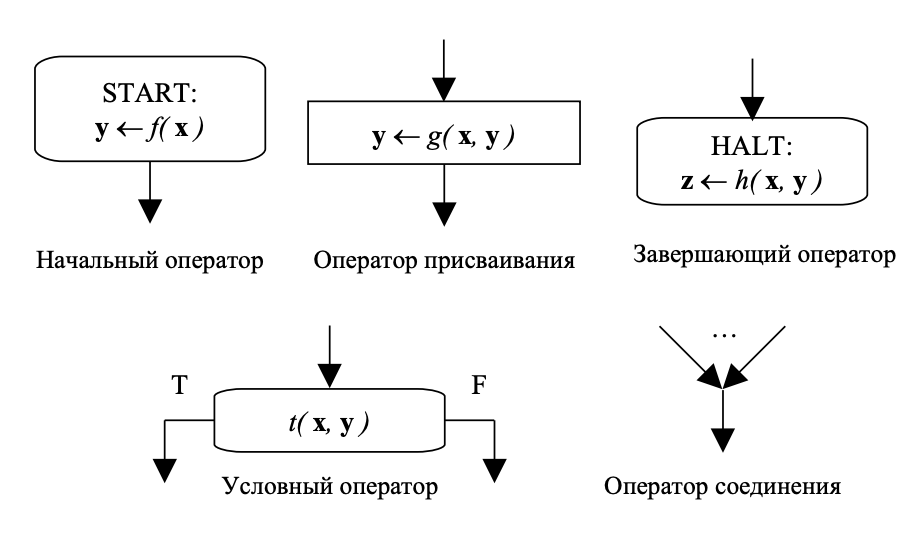
\includegraphics[scale=0.2]{pics/halt.png}

\textbf{Модель программы} - блок-схема. \textbf{Блок-схема} это тройка ( V, N, E ), где \textbf{V} – конечное множество переменных программы, \textbf{N} – конечное множество операторов блок-схемы, E $\subseteq$ N x \{ T, F, $\epsilon$ \} x N – конечное множество связок блок-схемы, помеченных символами T, F или $\epsilon$.

\textbf{Корректно-определенная блок-схема}:
\begin{enumerate}
    \item Ровно один начальный оператор и не менее одного завершающего оператора.
    \item Любой оператор находится на ориентированном пути от начального оператора к некоторому завершающему оператору.
    \item Число связок, выходящих из каждого оператора, и пометки этих связок соответствуют типу оператора: 
    \begin{itemize}
        \item Из начального оператора выходит ровно 1 дуга, помеченная символом $\epsilon$
        \item Из оператора присваивания выходит ровно 1 дуга, помеченная символом $\epsilon$.
        \item Из условного оператора выходит ровно 2 дуги, причем одна из них помечена символом T, а другая – символом F.
        \item Из оператора соединения выходит ровно 1 дуга, помеченная символом $\epsilon$.
        \item Из завершающего оператора не выходит ни одной дуги.
    \end{itemize}
    \item Число связок, входящих в каждый оператор, соответствует его типу
    \begin{itemize}
        \item В начальный оператор не входит ни одна дуга
        \item В оператор присваивания, условный и завершающий оператор входит ровно одна дуга
        \item В оператор соединения входит не менее одной дуги
    \end{itemize}
\end{enumerate}

\textbf{Определение}: $\forall$ оператора n и символа s в корректно-определенной блок-схеме (V, N, E) $\exists$ не более одного оператора n', что ( n, s, n' ) $\in$ E. Такой оператор n' (если он существует) мы будем называть \textit{последователем оператора} n по пометке s и обозначать как succ(n, s)

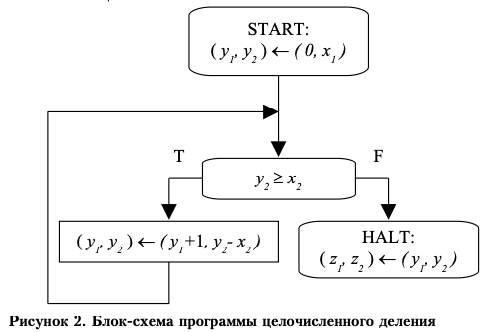
\includegraphics[scale=0.5]{pics/block_scheme.png}

\textbf{Конфигурацией программы} P будем называть пару ( \textit{l}, $\sigma$ ), где \textit{l} $\in$ $\lambda_P$ – метка текущего оператора программы, $\sigma$ =($d_1,d_2,...,d_{a+b}$ ) $\in$ $D_x^+$ x $D_y^+$ – вектор значений входных и промежуточных переменных программы.


Конечная или бесконечная последовательность конфигураций \{ $C_i$ | i=1,..,n,...\} программы P называется \textbf{вычислением}, если

\begin{enumerate}
    \item Метка первой конфигурации программы является меткой начального оператора.
    \item Значения всех входных переменных программы являются определенными ($\neq \omega$)  неизменными во всех конфигурациях вычисления.
    \item Значения промежуточных переменных в первой конфигурации равны $\omega$ (\textit{не определены}).
    \item Если метка $\textit{l}_i$ текущего оператора конфигурации $C_i$ является меткой начального оператора START: y $\leftarrow$ f(x), то следующая конфигурация $C_{i+1}$ состоит из метки оператора succ($n_i$, $\epsilon$) и вектора значений переменных $\sigma_{i+1} = \sigma_i[y \leftarrow f(x)]$.
    \item Если метка $\textit{l}_i$ текущего оператора конфигурации $C_i$ является меткой оператора присваивания ASSIGN: y $\leftarrow$ g(x, y), то следующая конфигурация $C_{i+1}$ состоит из метки оператора succ($n_i$, $\epsilon$) и вектора значений переменных $\sigma_{i+1} = \sigma_i[y \leftarrow g(x, y)]$..
    \item Если метка $\textit{l}_i$ текущего оператора конфигурации $C_i$ является меткой условного оператора TEST: t(x, y) и предикат t(x, y) при значениях переменных $\sigma_i$ принимает значение T, то следующая конфигурация $C_{i+1}$ состоит из метки оператора succ($n_i$, T) и вектора значений переменных $\sigma_{i+1} = \sigma_i$.
    \item Если метка $\textit{l}_i$ текущего оператора конфигурации $C_i$ является меткой условного оператора TEST: t(x, y) и предикат t(x, y) при значениях переменных $\sigma_i$ принимает значение F, то следующая конфигурация $C_{i+1}$ состоит из метки оператора succ($n_i$, F) и вектора значений переменных $\sigma_{i+1} = \sigma_i$.
    \item Если метка $\textit{l}_i$ текущего оператора конфигурации $C_i$ является меткой оператора соединения JOIN, то следующая конфигурация $C_{i+1}$ состоит из метки оператора succ($n_i$, $\epsilon$) и вектора значений переменных $\sigma_{i+1} = \sigma_i$.
    \item Если метка $\textit{l}_i$ текущего оператора конфигурации $C_i$ является меткой завершающего оператора HALT: z $\leftarrow$ h(x, y), то $C_i$ является последней конфигурацией вычисления.
    \item Если в конфигурации $C_{i+1}$ значение какой-либо промежуточной переменной равно $\omega$, то это последняя конфигурация вычисления.
\end{enumerate}

\textbf{Лемма}: Для каждой блок-схемы P и вектора значений ее входных переменных x существует единственное вычисление, в первой конфигурации которого значения входных переменных равны x.

